% ŠABLONA PRO PSANÍ ZÁVĚREČNÉ STUDIJNÍ PRÁCE
%%%%%%%%%%%%%%%%%%%%%%%%%%%%%%%%%%%%%%%%%%%%
% Autor: Jakub Dokulil (kubadokulil99@gmail.com)
% Tato šablona byla vytvořena tak, aby pomocí ní mohli v systému LaTeX soutěžící sázet své práce a zároveň odpovídala požadavkům na formátování vyplývajícím z wordové šablony umístěné na webu soc.cz.
%
\documentclass[12pt, a4paper,
%oneside,      %% -- odkomentujte, pokud chcete svou práci mít pouze jednostrannou, mezera pro hřbet pak automaticky bude pouze na levé straně
twoside,        %% -- pro oboustranné práce, mezera pro hřbet následně střídá strany.
openright
]{report}

%% Nutné balíčky a nastavení
%%%%%%%%%%%%%%%%%%%%%%%%%%%%

%% Proměnné
\newcommand\obor{INFORMAČNÍ TECHNOLOGIE} %% -- napiš číslo a název tvého oboru
\newcommand\kodOboru{18-20-M/01} %% -- napiš číslo a název tvého oboru
\newcommand\zamereni{se zaměřením na počítačové sítě a programování} %% -- napiš číslo a název tvého oboru
\newcommand\skola{Střední škola průmyslová a umělecká, Opava} %% vyplň název školy
\newcommand\trida{IT4} %% vyplň jméno svého konzultanta
\newcommand\jmenoAutora{Samuel Vaňuš}  %% vyplň své jméno
\newcommand\skolniRok{2023/24} %% vyplň rok
\newcommand\datumOdevzdani{1. 1. 2024} %% vyplň rok
\newcommand\nazevPrace{Inteligentní domácnost KNX} %% vyplň název své práce

\title{\nazevPrace} %% -- Název tvé práce
\author{\jmenoAutora} %% -- tvé jméno
\date{\datumOdevzdani} %% -- rok, kdy píšeš SOČku

\usepackage[top=2.5cm, bottom=2.5cm, left=3.5cm, right=1.5cm]{geometry} %% nastaví okraje, left -- vnitřní okraj, right -- vnější okraj

\usepackage[czech]{babel} %% balík babel pro sazbu v češtině
\usepackage[utf8]{inputenc} %% balíky pro kódování textu
\usepackage[T1]{fontenc}
\usepackage{cmap} %% balíček zajišťující, že vytvořené PDF bude prohledávatelné a kopírovatelné

\usepackage{graphicx} %% balík pro vkládání obrázků

\usepackage{caption}
\usepackage{subcaption} %% balíček pro vkládání podobrázků

\usepackage{hyperref} %% balíček, který v PDF vytváří odkazy

\linespread{1.25} %% řádkování
\setlength{\parskip}{0.5em} %% odsazení mezi odstavci


\usepackage[pagestyles]{titlesec} %% balíček pro úpravu stylu kapitol a sekcí
\titleformat{\chapter}[block]{\scshape\bfseries\LARGE}{\thechapter}{10pt}{\vspace{0pt}}[\vspace{-22pt}]
\titleformat{\section}[block]{\scshape\bfseries\Large}{\thesection}{10pt}{\vspace{0pt}}
\titleformat{\subsection}[block]{\bfseries\large}{\thesubsection}{10pt}{\vspace{0pt}}


\usepackage{tocloft} % Balíček umožní přizpůsobit vzhled tabulky obsahu
\setlength{\cftbeforechapskip}{0pt}  % Menší rozestup pro kapitoly
\setlength{\cftbeforesecskip}{0pt}   % Menší rozestup pro sekce

\setcounter{secnumdepth}{2}
\setcounter{tocdepth}{1}
\usepackage{fancyhdr}
\pagestyle{fancy}
\renewcommand{\headrulewidth}{0.025pt}

\usepackage{booktabs}

\usepackage{url}

%% Balíčky co se můžou hodit :) 
%%%%%%%%%%%%%%%%%%%%%%%%%%%%%%%

\usepackage{pdfpages} %% Balíček umožňující vkládat stránky z PDF souborů, 

\usepackage{upgreek} %% Balíček pro sazbu stojatých řeckých písmen, třeba u jednotky mikrometr. Například stojaté mí: \upmu, stojaté pí: \uppi

\usepackage{amsmath}    %% Balíčky amsmath a amsfonts 
\usepackage{amsfonts}   %% pro sazbu matematických symbolů
\usepackage{esint}     %% pro sazbu různých integrálů (např \oiint)
\usepackage{mathrsfs}
\usepackage{helvet} % Helvet font
\usepackage{mathptmx} % Times New Roman
\usepackage{Oswald} % Oswald font
\usepackage{pdfpages}


%% makra pro sazbu matematiky
\newcommand{\dif}{\mathrm{d}} %% makro pro sazbu diferenciálu, místo toho
%% abych musel psát '\mathrm{d}' mi stačí napsat '\dif' což je mnohem 
%% kratší a mohu si tak usnadnit práci

\usepackage{listings}
\usepackage{xcolor}

\renewcommand{\lstlistingname}{Kód}% Listing -> Algorithm
\renewcommand{\lstlistlistingname}{Seznam programových kódů}% List of Listings -> List of Algorithms

%% Definice 
\lstdefinelanguage{JavaScript}{
	morekeywords=[1]{break, continue, delete, else, for, function, if, in,
		new, return, this, typeof, var, void, while, with},
	% Literals, primitive types, and reference types.
	morekeywords=[2]{false, null, true, boolean, number, undefined,
		Array, Boolean, Date, Math, Number, String, Object},
	% Built-ins.
	morekeywords=[3]{eval, parseInt, parseFloat, escape, unescape},
	sensitive,
	morecomment=[s]{/*}{*/},
	morecomment=[l]//,
	morecomment=[s]{/**}{*/}, % JavaDoc style comments
	morestring=[b]',
	morestring=[b]"
}[keywords, comments, strings]


\lstdefinelanguage[ECMAScript2015]{JavaScript}[]{JavaScript}{
	morekeywords=[1]{await, async, case, catch, class, const, default, do,
		enum, export, extends, finally, from, implements, import, instanceof,
		let, static, super, switch, throw, try},
	morestring=[b]` % Interpolation strings.
}

\lstalias[]{ES6}[ECMAScript2015]{JavaScript}

% Nastavení barev
% Requires package: color.
\definecolor{mediumgray}{rgb}{0.3, 0.4, 0.4}
\definecolor{mediumblue}{rgb}{0.0, 0.0, 0.8}
\definecolor{forestgreen}{rgb}{0.13, 0.55, 0.13}
\definecolor{darkviolet}{rgb}{0.58, 0.0, 0.83}
\definecolor{royalblue}{rgb}{0.25, 0.41, 0.88}
\definecolor{crimson}{rgb}{0.86, 0.8, 0.24}

% Nastavení pro Python
\lstdefinestyle{Python}{
	language=Python,
	backgroundcolor=\color{white},
	basicstyle=\ttfamily,
	breakatwhitespace=false,
	breaklines=false,
	captionpos=b,
	columns=fullflexible,
	commentstyle=\color{mediumgray}\upshape,
	emph={},
	emphstyle=\color{crimson},
	extendedchars=true,  % requires inputenc
	fontadjust=true,
	frame=single,
	identifierstyle=\color{black},
	keepspaces=true,
	keywordstyle=\color{mediumblue},
	keywordstyle={[2]\color{darkviolet}},
	keywordstyle={[3]\color{royalblue}},
	literate=%
	{á}{{\'a}}1 {č}{{\v{c}}}1 {ď}{{\v{d}}}1 {é}{{\'e}}1 {ě}{{\v{e}}}1
	{í}{{\'i}}1 {ň}{{\v{n}}}1 {ó}{{\'o}}1 {ř}{{\v{r}}}1 {š}{{\v{s}}}1
	{ť}{{\v{t}}}1 {ú}{{\'u}}1 {ů}{{\r{u}}}1 {ý}{{\'y}}1 {ž}{{\v{z}}}1,		
	numbers=left,
	numbersep=5pt,
	numberstyle=\tiny\color{black},
	rulecolor=\color{black},
	showlines=true,
	showspaces=false,
	showstringspaces=false,
	showtabs=false,
	stringstyle=\color{forestgreen},
	tabsize=2,
	title=\lstname,
	upquote=true  % requires textcomp	
}


\lstdefinestyle{JSES6Base}{
	backgroundcolor=\color{white},
	basicstyle=\ttfamily,
	breakatwhitespace=false,
	breaklines=false,
	captionpos=b,
	columns=fullflexible,
	commentstyle=\color{mediumgray}\upshape,
	emph={},
	emphstyle=\color{crimson},
	extendedchars=true,  % requires inputenc
	fontadjust=true,
	frame=single,
	identifierstyle=\color{black},
	keepspaces=true,
	keywordstyle=\color{mediumblue},
	keywordstyle={[2]\color{darkviolet}},
	keywordstyle={[3]\color{royalblue}},
 literate=%
{á}{{\'a}}1 {č}{{\v{c}}}1 {ď}{{\v{d}}}1 {é}{{\'e}}1 {ě}{{\v{e}}}1
{í}{{\'i}}1 {ň}{{\v{n}}}1 {ó}{{\'o}}1 {ř}{{\v{r}}}1 {š}{{\v{s}}}1
{ť}{{\v{t}}}1 {ú}{{\'u}}1 {ů}{{\r{u}}}1 {ý}{{\'y}}1 {ž}{{\v{z}}}1,		
	numbers=left,
	numbersep=5pt,
	numberstyle=\tiny\color{black},
	rulecolor=\color{black},
	showlines=true,
	showspaces=false,
	showstringspaces=false,
	showtabs=false,
	stringstyle=\color{forestgreen},
	tabsize=2,
	title=\lstname,
	upquote=true  % requires textcomp
}

\lstdefinestyle{JavaScript}{
	language=JavaScript,
	style=JSES6Base,
}
\lstdefinestyle{ES6}{
	language=ES6,
	style=JSES6Base
}


%% Bordel pro práci - můžeš smáznout :) 
%%%%%%%%%%%%%%%%%%%

\usepackage{lipsum} %% balíček který píše lipsum (nesmyslný text, který se používá pro kontrolu typografie)

%% Začátek dokumentu
%%%%%%%%%%%%%%%%%%%%
\begin{document}
	
	\pagestyle{empty}
	\pagenumbering{Roman}
	
	\cleardoublepage

%% Titulní stránka s informacemi
%%%%%%%%%%%%%%%%%%%%%%%%%%%%%%%%%%%%%%%%
	
	{\fontfamily{phv}\selectfont
		%% Logo školy
		\begin{figure}[h]
			\centering
			
\includegraphics[width=0.6\linewidth]{image/logo-skoly.png} 
		\end{figure}
		
		
		%% Hlavička práce a její název (viz proměnná \nazev prace)
		%% \sffamily %%% bezpatkové písmo - sans serif
		{\bfseries %%% písmo na stránce je tučně
			\begin{center}
				\vspace{0.025 \textheight}
				\LARGE{ZÁVĚREČNÁ STUDIJNÍ PRÁCE}\\
				\large{dokumentace}\\
				\vspace{0.075 \textheight}
				\LARGE {\nazevPrace}\\
			\end{center}  
		}%%%
		
		\begin{figure}[h]
			\centering
			
\includegraphics[width=0.6\linewidth]{image/smart_home.jpg} 
		\end{figure}
		
		\vspace{0.02 \textheight}
		\begin{table}[h!]
			\begin{tabular}{ll}
				\textbf{Autor:} & \jmenoAutora\\ 
				\textbf{Obor:} & \kodOboru { } \obor\\
				\textbf{} & \zamereni\\
				\textbf{Třída:} & \trida\\
				\textbf{Školní rok:} & \skolniRok\\
			\end{tabular}
			
		\end{table}		
	}
	
\cleardoublepage %% Zalomení dvojstránky
	
%% Stránka obsahující poděkování a prohlášení
%%%%%%%%%%%%%%%%%%%%%%%%%%%%%%%%%%%%%%%%%%%%%%%%%%%%%%%%

%% Poděkování - nepovinné
%%%%%%%%%%%%%%%%%%%%%%%%%%%%
	
	\noindent{\large{\bfseries{Poděkování}\\}}
	\noindent \textit {Rád bych poděkoval doc. Ing. Janu Vaňušovi, Ph.D., za vedení při této práci a poskytnutí veškerých využitých zařízení a podkladových materiálů.}
	
	\vspace*{0.7\textheight} %% Vertikální mezeru je možné upravit

%% Prohlášení - povinné
%%%%%%%%%%%%%%%%%%%%%%%%%%%%
	\noindent{\large{\bfseries{Prohlášení}\\}}  %% uprav si koncovky podle toho na jaký rod se cítíš, vypadá to pak lépe :) 
	\noindent{Prohlašuji, že jsem závěrečnou práci vypracoval samostatně a uvedl veškeré použité 
		informační zdroje.\\}
	\noindent{Souhlasím, aby tato studijní práce byla použita k výukovým a prezentačním účelům na Střední průmyslové a umělecké škole v Opavě, Praskova 399/8.}
	\vfill
	\noindent{V Opavě \datumOdevzdani\\}
	\noindent
	\begin{minipage}{\linewidth}
		\hspace{9.5cm} 
		\begin{tabular}{@{}p{6cm}@{}}
			\dotfill \\
			Podpis autora
		\end{tabular}
	\end{minipage}
	
	\cleardoublepage 
	\noindent{\Large{\bfseries{Anotace}\\}}
	\noindent Práce předvádí systém inteligentní domácnosti KNX, konkrétně zařízení pracující s tímto systémem a vizualizační prostředí. Popisuje konfiguraci zařízení, vlastnosti zařízení a následnou vizualizaci finálního systému. Výsledek je zpracován pomocí aplikace ETS6 a je vizuálně zobrazitelný pomocí komerčního software Wiser, Uživatel může zhasínat a rozsvěcovat přepínací a stmívací světla, ovládat pozici žaluzií, zapnout topný systém stylu FanCoil, detekovat objem CO2 a vlhkost v ovzduší, teplotu a přítomnost v místnosti z chytrého telefonu nebo počítače. 	
	
	\vspace{18pt}
	
	\noindent{\large{\bfseries{Klíčová slova}}}
	
	\noindent Akční člen, skupinová adresa, vizualizace, konfigurace, scéna, inteligentní domácnost\dots 
	
	\vspace{18pt}
	
	\clearpage %% Zalomení stránky

%% Stránka s generovaným obsahem
%%%%%%%%%%%%%%%%%%%%%%%%%%%%%%%%%%%%%%%	
	
	\tableofcontents %% Vygeneruje tabulku s obsahem

	\pagenumbering{arabic} %% Nastavení způsobu číslování stránek (alternativy roman | Roman)
	\setcounter{page}{1} %% Nastavení počitadla stránek

%% Stránka s úvodem - povinná část
%%%%%%%%%%%%%%%%%%%%%%%%%%%%%%%%%%%%%%%		
	\chapter*{Úvod}
%Tento příkaz vytvoří novou kapitolu s názvem "Úvod" ve vašem dokumentu.
%Hvězdička * u příkazu \chapter* znamená, že tato kapitola nebude mít číslo. Ve výsledném dokumentu se tedy objeví jako "Úvod" bez předcházejícího čísla kapitoly, které se obvykle zobrazuje u číslovaných kapitol.
%Tento příkaz také znamená, že kapitola se automaticky neobjeví v obsahu, protože LaTeX standardně zahrnuje do obsahu pouze číslované kapitoly.
	\addcontentsline{toc}{chapter}{Úvod}
%Tento příkaz ručně přidává záznam do obsahu.
%První parametr toc označuje, že přidáváme záznam do Table of Contents (obsahu).
%Druhý parametr chapter specifikuje úroveň záznamu. V tomto případě říkáme, že přidávaný záznam má být považován za kapitolu.
%Třetí parametr Úvod je text, který se objeví v obsahu. V tomto případě bude v obsahu zobrazen název "Úvod".	
Cílem práce byla konfigurace zařízení výukového modelu plně vybaveného zařízeními pro fungování 2+kk bytu a následné nastavení vizualizačního prostředí optimálně spolu s následnou tvorbou prostředí vlastního. Využil jsem aplikaci ETS6, se kterou jsem se seznámil na odborných praxích ve třetím ročníku.
Hlavní motivací bylo sebezdokonalení se v práci s touto technologií pro možné využití v mém následném vzdělání. Poptávka po odbornících v oboru inteligentní domácnosti rovněž v posledních letech vzrostla, což opět rozšiřuje můj výběr budoucího zaměstnání.
Tato práce nejprve obeznamuje s použitou technologií a vysvětluje výhody a nevýhody různých řešení inteligentní domácnosti. Dále se věnuje konfiguraci pomocí ETS6 a následné nahrávání do jednotlivých zařízení.
V další části předvádí vizualizační prostředí vytvořené pomocí Wiseru. Rovněž vysvětluje základy práce pomocí tohoto software a předvádí výsledné prostředí, kterého je možno jednoduše dosáhnout, komplikace, které mohou nastat a splněné a nesplněné cíle práce.


%Tipy k psaní úvodu
%Je povinný, nadpis neměňte, rozsah - max. 1 strana. 
%Tato část práce obsahuje: 
%* náhled do řešené problematiky, zdůvodnění volby problematiky, 
%* předem definované cíle práce, 
%* motivaci pro další čtení textu včetně stručného uvedení obsahu následujících kapitol 


\chapter{Technologie}

\section{O KNX}
\label{sec:uvod}

Technologie \textbf {KNX} \cite{KNX} je jednou z nejrozšířenějších technologií pro funkci inteligentní domácnosti. Umožňuje ovládat a monitorovat různé prvky domácnosti, jako jsou světla, žaluzie, topení, zásuvky atd. pomocí různých displayů, ovladačů, ale i osobních zařízení. Konkurují ji např. Loxone\cite{Loxone}, Home assistant \cite{HA}, BACnet\cite{BAC}, LonWorks\cite{LW}, český Teco\cite{Teco} nebo iNELS\cite{INELS}.
\subsection{Co to je KNX}
KNX je organizace s cílem vytvoření otevřeného standardu pro aplikace pro inteligentní budovy, obchodní značky zahrnující pod sebe přístroje od různých dodavatelů, stanovení KNX jako celosvětové normy a podpory vzdělávacích aktivit a školení pro práci s tímto systémem. Pro konfiguraci zařízení je využíván komerční software \textbf {ETS}, který se neustále vyvíjí.  Všechny produkty pod značkou KNX jsou navzájem kompatibilní a mají vlastní firmware, díky čemuž je celý systém \textbf {decentralizovaný}.


\section{Výhody a nevýhody technologie}
Hlavní výhodou je snadná dostupnost a možnost zakombinování dalších systémů do celkového projektu. Mezi další výhody patří: 

\begin{itemize}
	\item Decentralizovaná struktura zajišťující flexibilitu, ochranu před selháním na základě poruchy jednoho zařízení, rychlost komunikace apod.
	\item Otevřenost standardu, což znamená že zařízení různých výrobců jsou stále kompatibilní.
	\item Úspornost z pohledu spotřeby energie s možností nastavení doplňkových scén za účelem dalšího snížení spotřeby.
	\item Jednoduchá instalace a konfigurace.
	\item Množství školicích center
	\item Několik různých možností propojení zařízení.
\end{itemize}

I přes tyto výhody ale existují i problémy, jako: 

\begin{itemize}
	\item Cena přístrojů v porovnání s jinými systémy.
	\item Pro již postavené domy může být náročnější instalace.
	\item U větších projektů je potřeba odborné znalosti, kvůli čemuž bude třeba počítat s možností nechat se zaškolit nebo si najmout odborníka.
\end{itemize}

\chapter{Hardware}

\section{Použitá zařízení}
\label{sec:hw_devices}

V této kapitole se nachází výčet a vlastnosti jednotlivých zařízení, jako jsou vypínače, akční členy, senzory apod.

\includepdf[pages={2}]{attachments/Topology.pdf}

\begin{figure}[h]
\subsection{Technický popis přístrojů}
\centering
\begin{subfigure}{0.85\textwidth}
	\subsubsection{KNX DALI brána}
	DALI je individuální systém pro osvětlení. Pro propojení se systémem KNX je tedy potřeba přístroj jako tato brána, který tvoří rozhraní mezi oběmi směrnicemi. Tento přístroj může ovládat až 64 výstupů v šestnácti skupinách a kontrolovat až 16 jednotlivých scén. Jedná se o volně konfigurovatelné zařízení obsahující pouze jeden controler, kvůli čemuž nemůže využít snímače DALI-2, mezi které patří např. detektory pohybu, přítomnosti apod.


	\noindent V mém projektu je pomocí tohoto přístroje ovládáno stmívané světlo v koupelně.


		\centering
		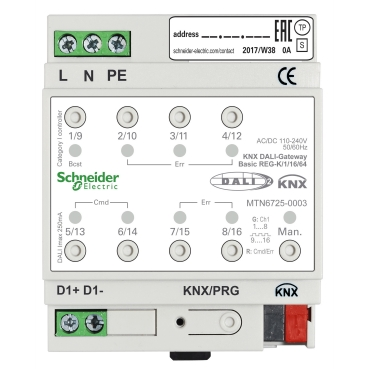
\includegraphics[scale=0.34]{image/MTN6725-0003.jpg}
		\caption{MTN6725-0003}
		\label{image:1}
\end{subfigure}

\begin{subfigure}{0.85\textwidth}
	\subsubsection{Akční spínací člen MTN649204}
	Akční člen je prvek, který zpracovává informace a převádí je do technické fáze, tj. ovládá konečné zařízení, jako je žárovka, žaluzie apod. Tento konkrétní přístroj může ovládat až 4 prvky, a to i pomocí manuálního modu, který je možno spustit pomocí malého černého tlačítka pod LED s označením "Hand", a který odblokuje ostatní čtyři tlačítka na desce přístroje, přičemž každé ovládá jeden výstup. Zařízení nemá předem nahranou pevnou konfiguraci, takže je rovněž volně konfigurovatelné.Prodej byl ukončen v srpnu 2023.


	\noindent Zde je napojeno na 4 led žárovky symbolizující zásuvky rozmístěné různě v objektu.


		\centering
		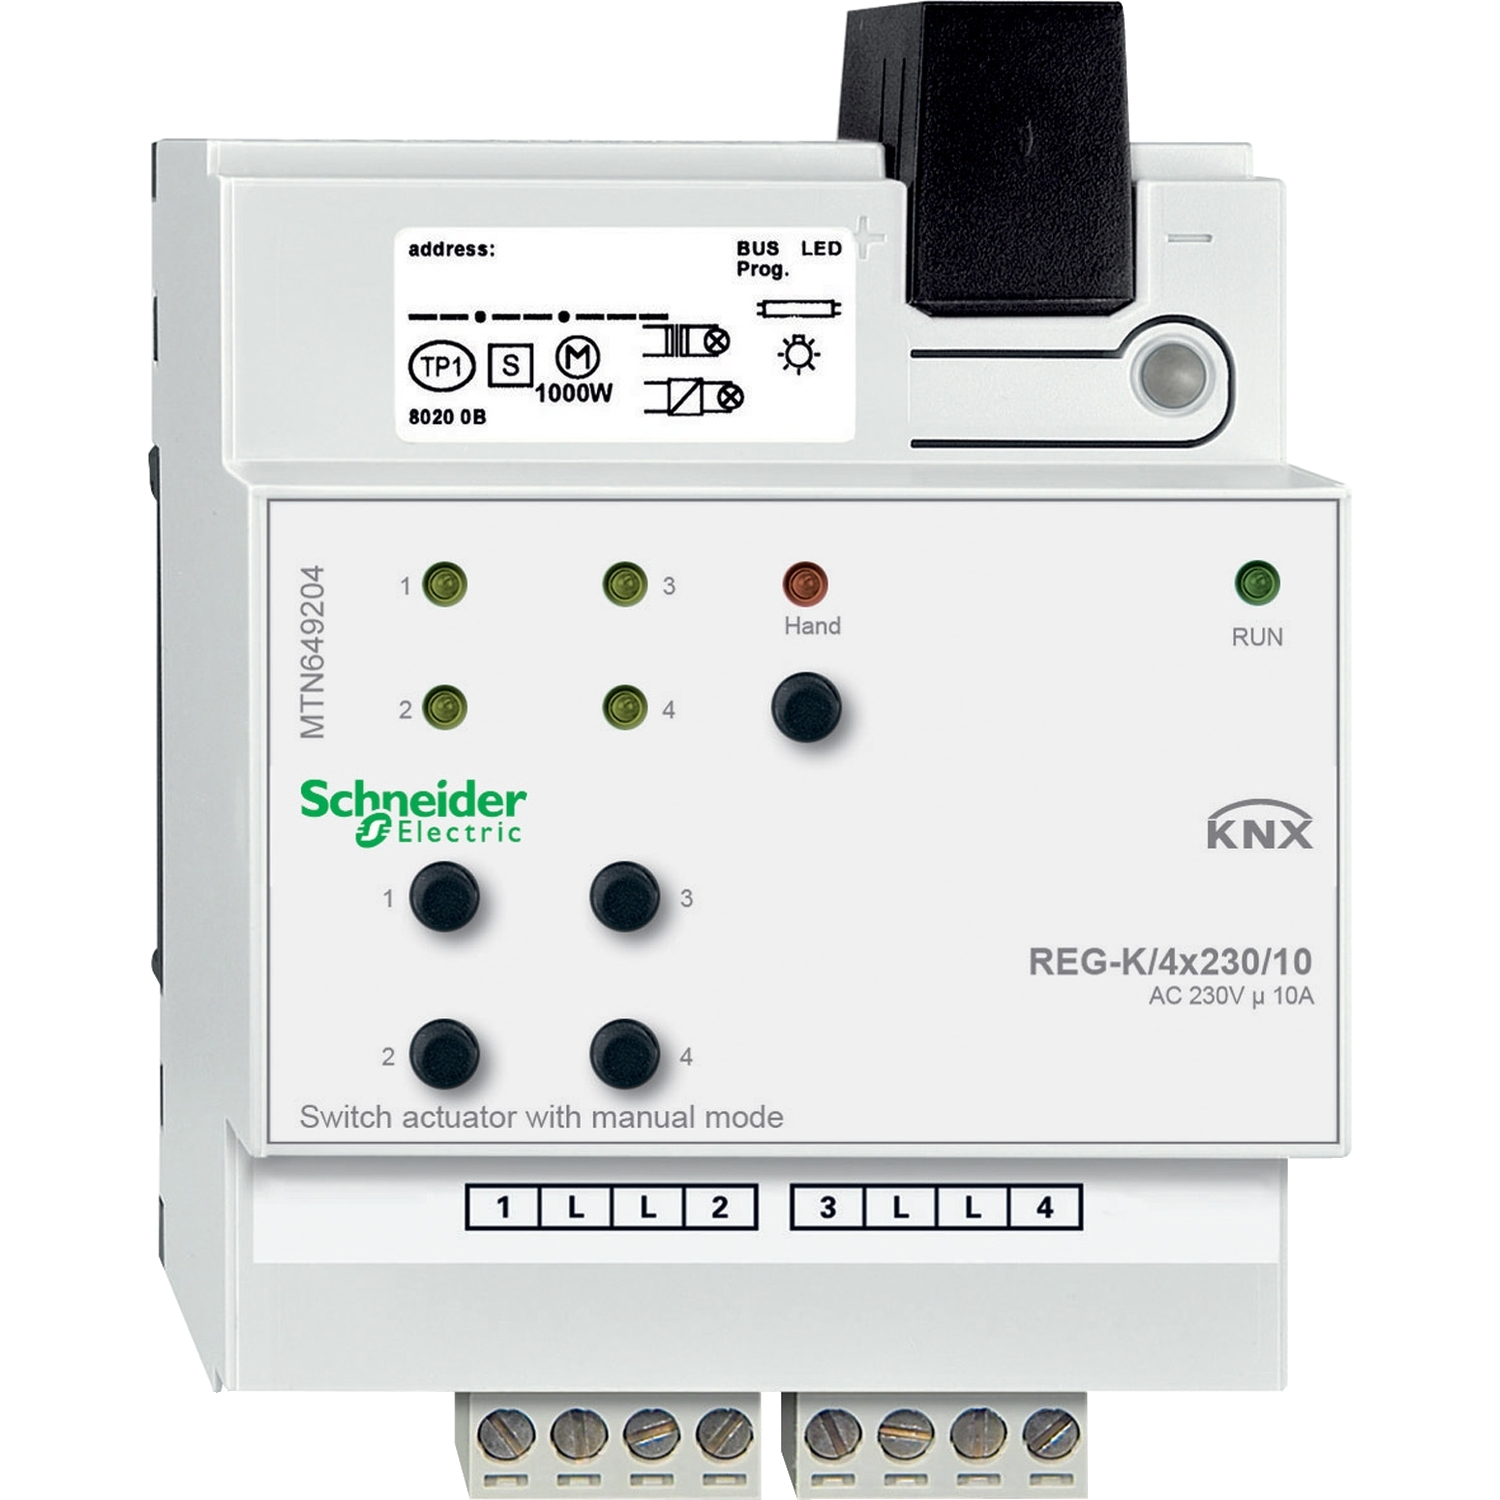
\includegraphics[scale=0.085]{image/MTN649204.jpg}
		\caption{MTN649204}
		\label{image:2}
\end{subfigure}
\end{figure}

\begin{figure}[h]
\centering
\begin{subfigure}{0.9\textwidth}
	\subsubsection{Akční člen žaluzií MTN649804}
	Jedná se o akční člen s možností ovládání až čtyř pohonů žaluzií. Zařízení také poskytuje volnou konfiguraci a manuální mod se signálními LED.


	\noindent V tomto projektu je využito všech čtyř výstupů, samotné žaluzie jsou však předstvovány přepínacímí šipkami reprezentujícími směr pohybu žaluzií.
 
		\centering
		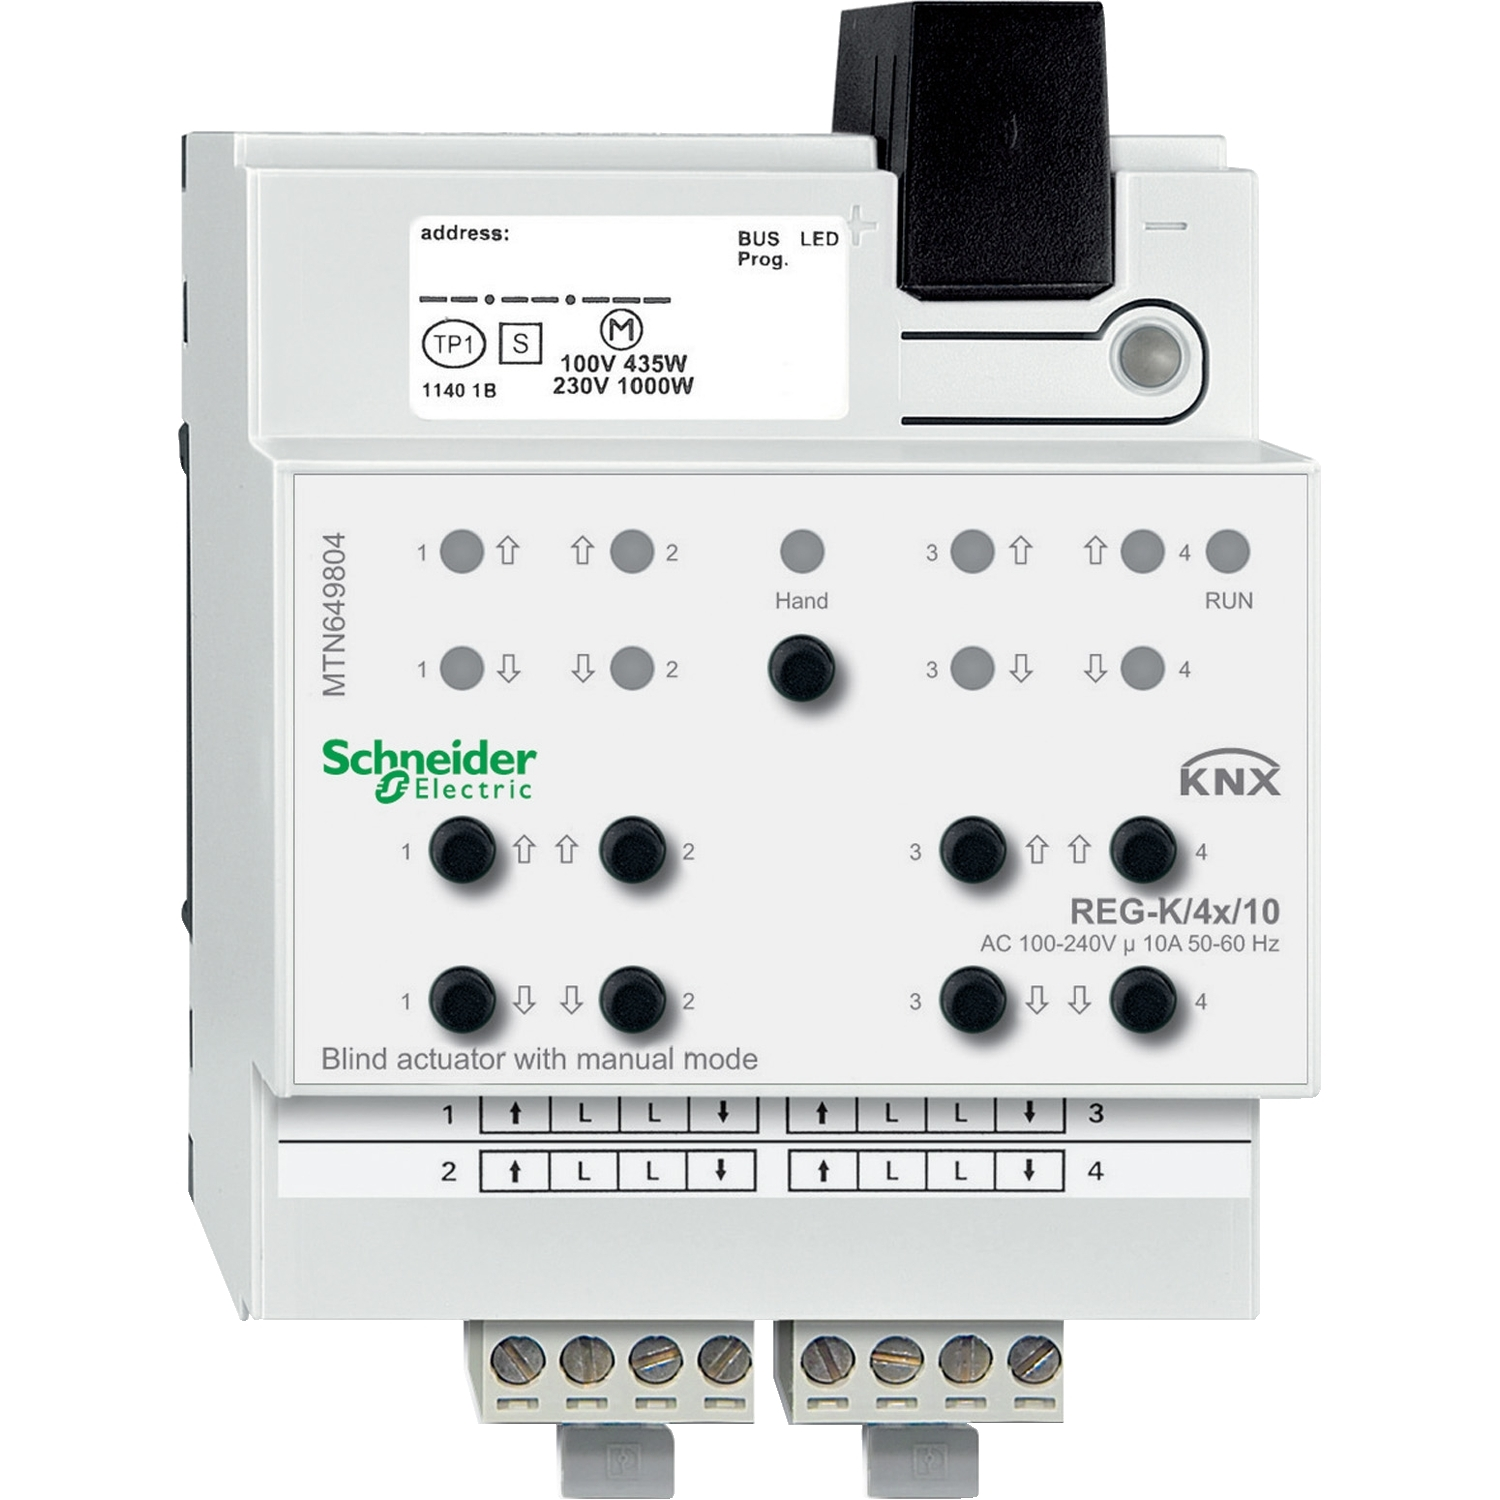
\includegraphics[scale=0.09]{image/MTN649804.jpg}
		\caption{MTN649804}
		\label{image:3}
\end{subfigure}

\begin{subfigure}{0.9\textwidth}
	\subsubsection{Kontrolní jednotka MTN646991}
	Tato kontrolní jednotka má k dispozici tři výstupy s rozhraním 0-10 V a variantou manuálního ovládání v podobě páčkových přepínačů. Jedná se opět o volně konfigurovatelný přístroj.


	\noindent Pomocí této jednotky jsou ovládány další tři světla, která mají možnost stmívání znázorněnou hodnotami voltmetrů u každé žárovky.

		\centering
		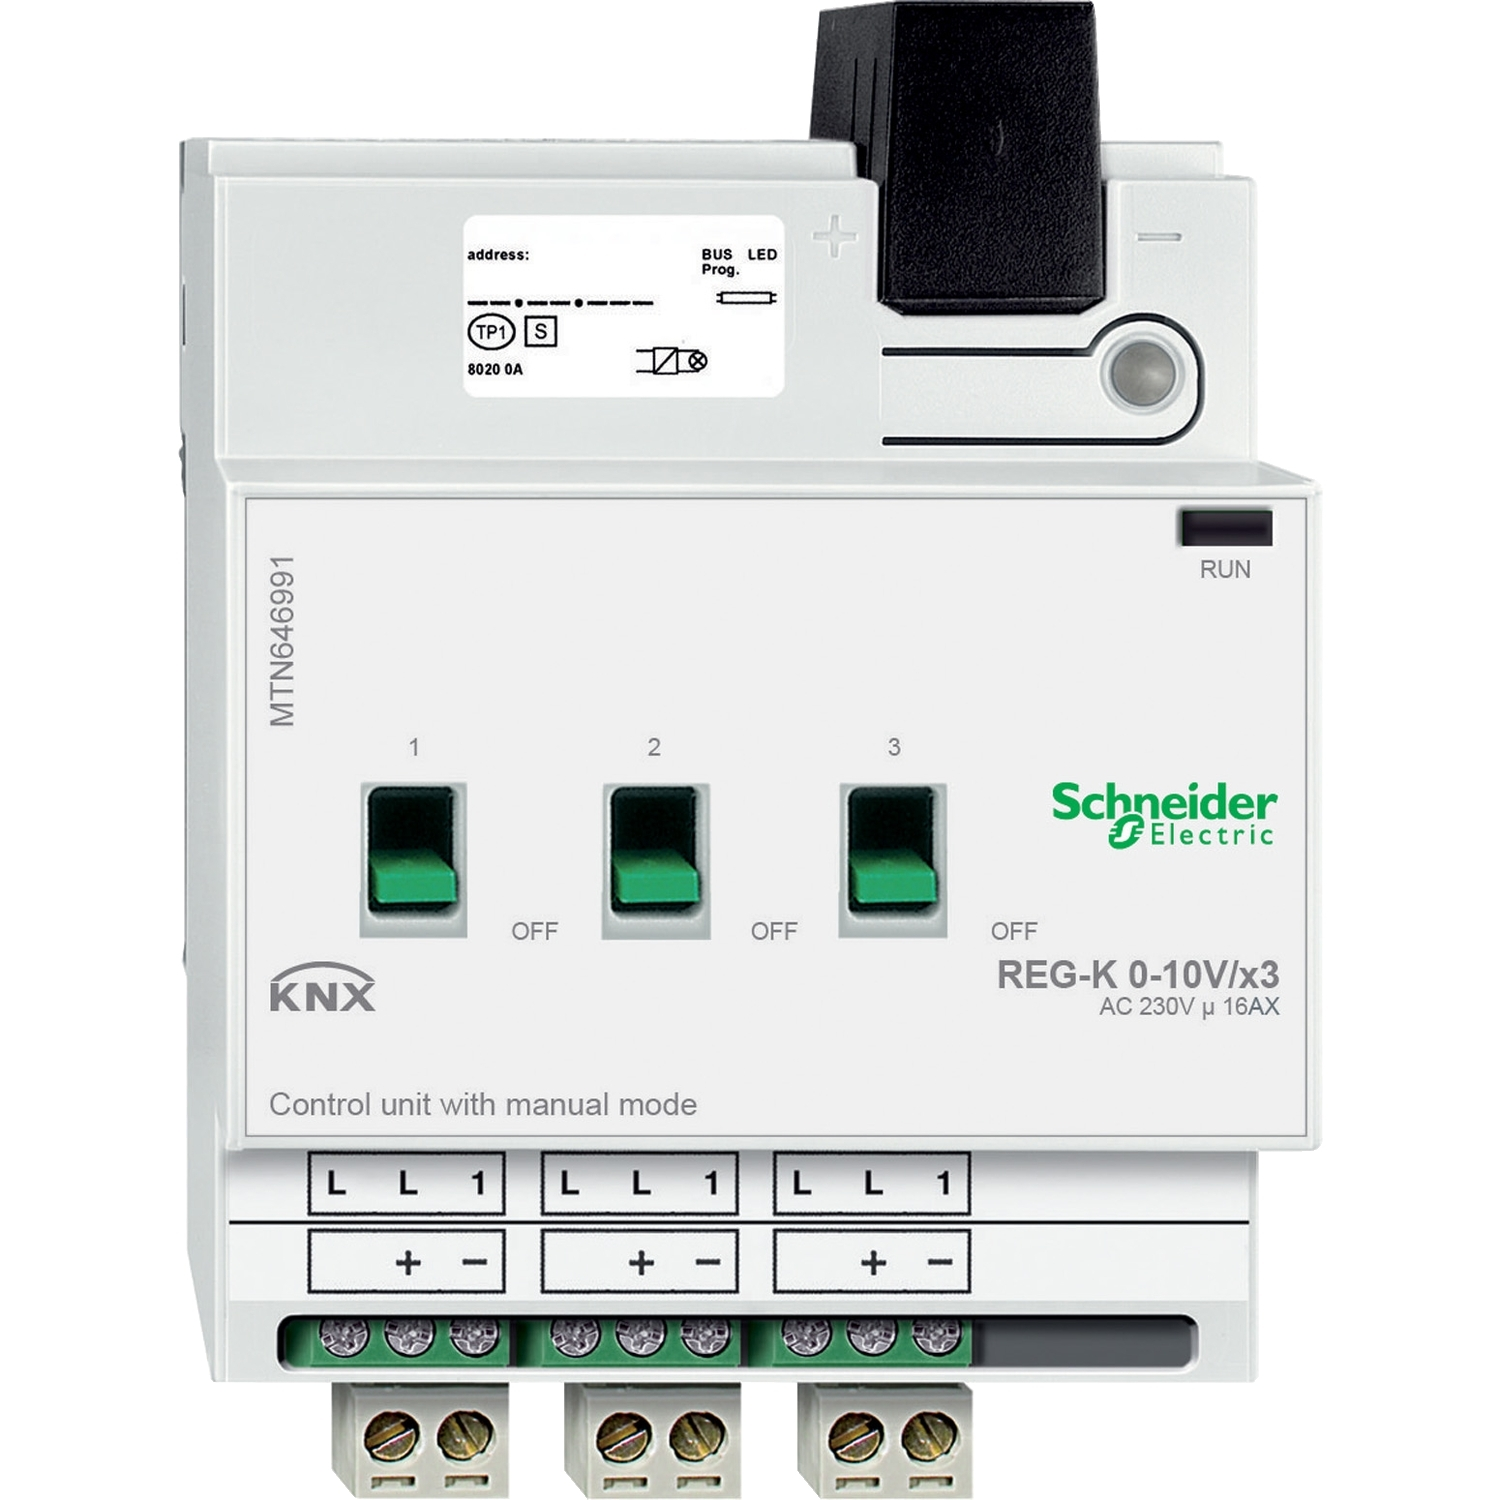
\includegraphics[scale=0.09]{image/MTN646991.jpg}
		\caption{MTN646991}
		\label{image:4}
\end{subfigure}
\end{figure}


\begin{figure}[h]
\centering
\begin{subfigure}{0.9\textwidth}
	\subsubsection{Akční člen FAN coil}
	Fan coil jednotky jsou zařízení sloužící k řízení specifického systému vytápění. Tento systém funguje na principu vytváření proudu vzduchu tvořeného pomocí ventilátoru, odtud "Fan", přes výměník tepla, neboli několik vrstev potrubí do kterého je vedena voda s potřebnou teplotou. Odtud pak "coil". Existují Fan coil systémy, dvoutrubkový, který má přívodní a odtokovou trubku, do kterých je vedena i studená i teplá voda, a čtyřtrubkový, ve kterém je samostatný výměník pro ohřívání a chlazení.


	\noindent Zařízení použito v tomto projektu podporuje obě varianty, přičemž nastavena je čtyřtrubková. Ventilátor pak disponuje až třemi rychlostmi. Zařízení je opět volně konfigurovatelné s možností příjmu dat ze senzorů otevření oken, výšky hladiny nádrže apod.l
		\centering
		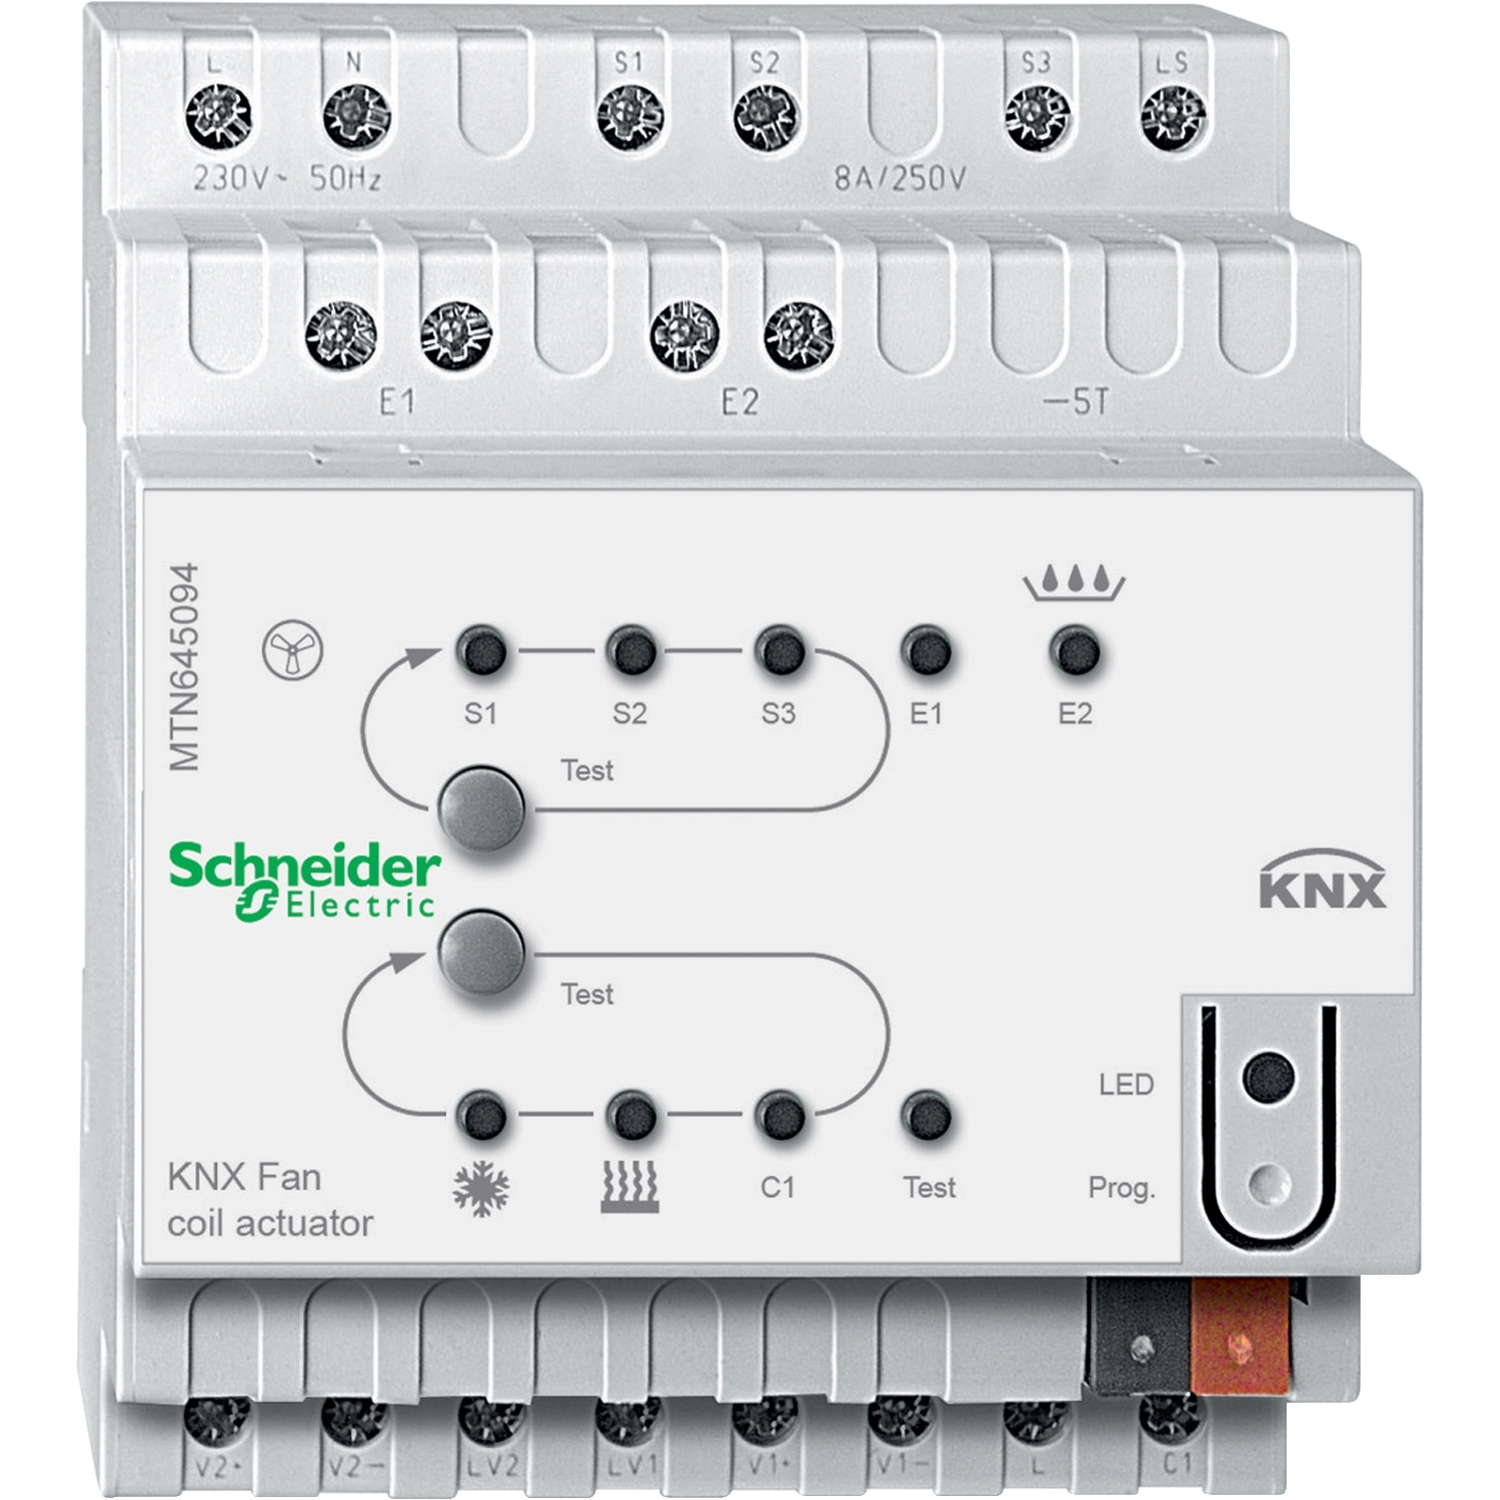
\includegraphics[scale=0.09]{image/MTN645094.jpg}
		\caption{MTN645094}
		\label{image:5}
		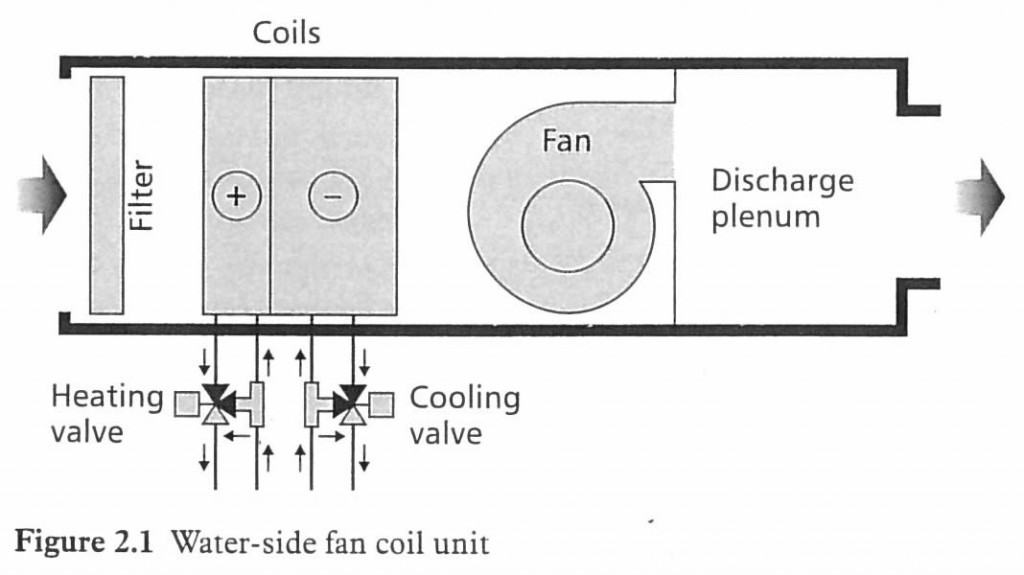
\includegraphics[scale=0.2]{image/fancoil.jpg}
		\caption{Obecný princip Fan coil}
		\label{img:6}
\end{subfigure}

\begin{subfigure}{0.9\textwidth}
	\subsubsection{USB rozhraní  MTN6502-0101}
	Pomocí tohoto rozhraní lze připojit přístroj používaný pro konfiguraci ke sběrnici pomocí konektoru USB-C. Další možností spojení je například mnou používaný Ethernet (KNX IP).
		\centering
		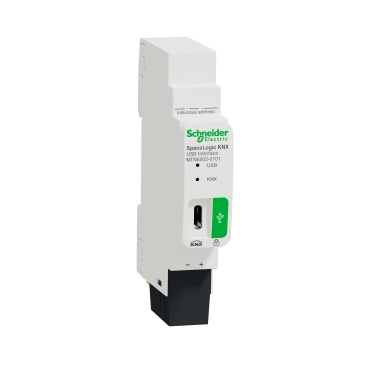
\includegraphics[scale=0.2]{image/MTN6502-0101.jpg}
		\caption{MTN6502-0101}
		\label{image:7}
\end{subfigure}
\end{figure}

\begin{figure}[h]
\centering
\begin{subfigure}{0.9\textwidth}
	\subsubsection{SpaceLogic KNX spojka}
	Toto zařízení slouží k řízení logického vztahu linie a oblasti (liniová spojka) nebo oblasti a páteřní oblasti (oblastní spojka) s možností zabezpečení KNX aktivovatelnou pomocí ETS. Pomocí tabulky filtrů rozlišuje, které telegramy projdou na vedlejší linii a které nebudou využity a tudíž nejsou potřeba předávat. Je možné filtrační tabulku úplně vypnout, čímž spojka začne zastávat roli opakovače, což znamená že můžeme ke stávajícímu segmentu připojit až další dva, přičemž každý pojme maximálně 64 individuálních adres.

	\noindent V tomto projektu je toto zařízení nastaveno jako liniová spojka bez většího zabezpečení mezi oblastí 5.x.x a linií 5.1.x, a prot, i z důvodu přehlednosti topologie, disponuje adresou 5.1.0.
		\centering
		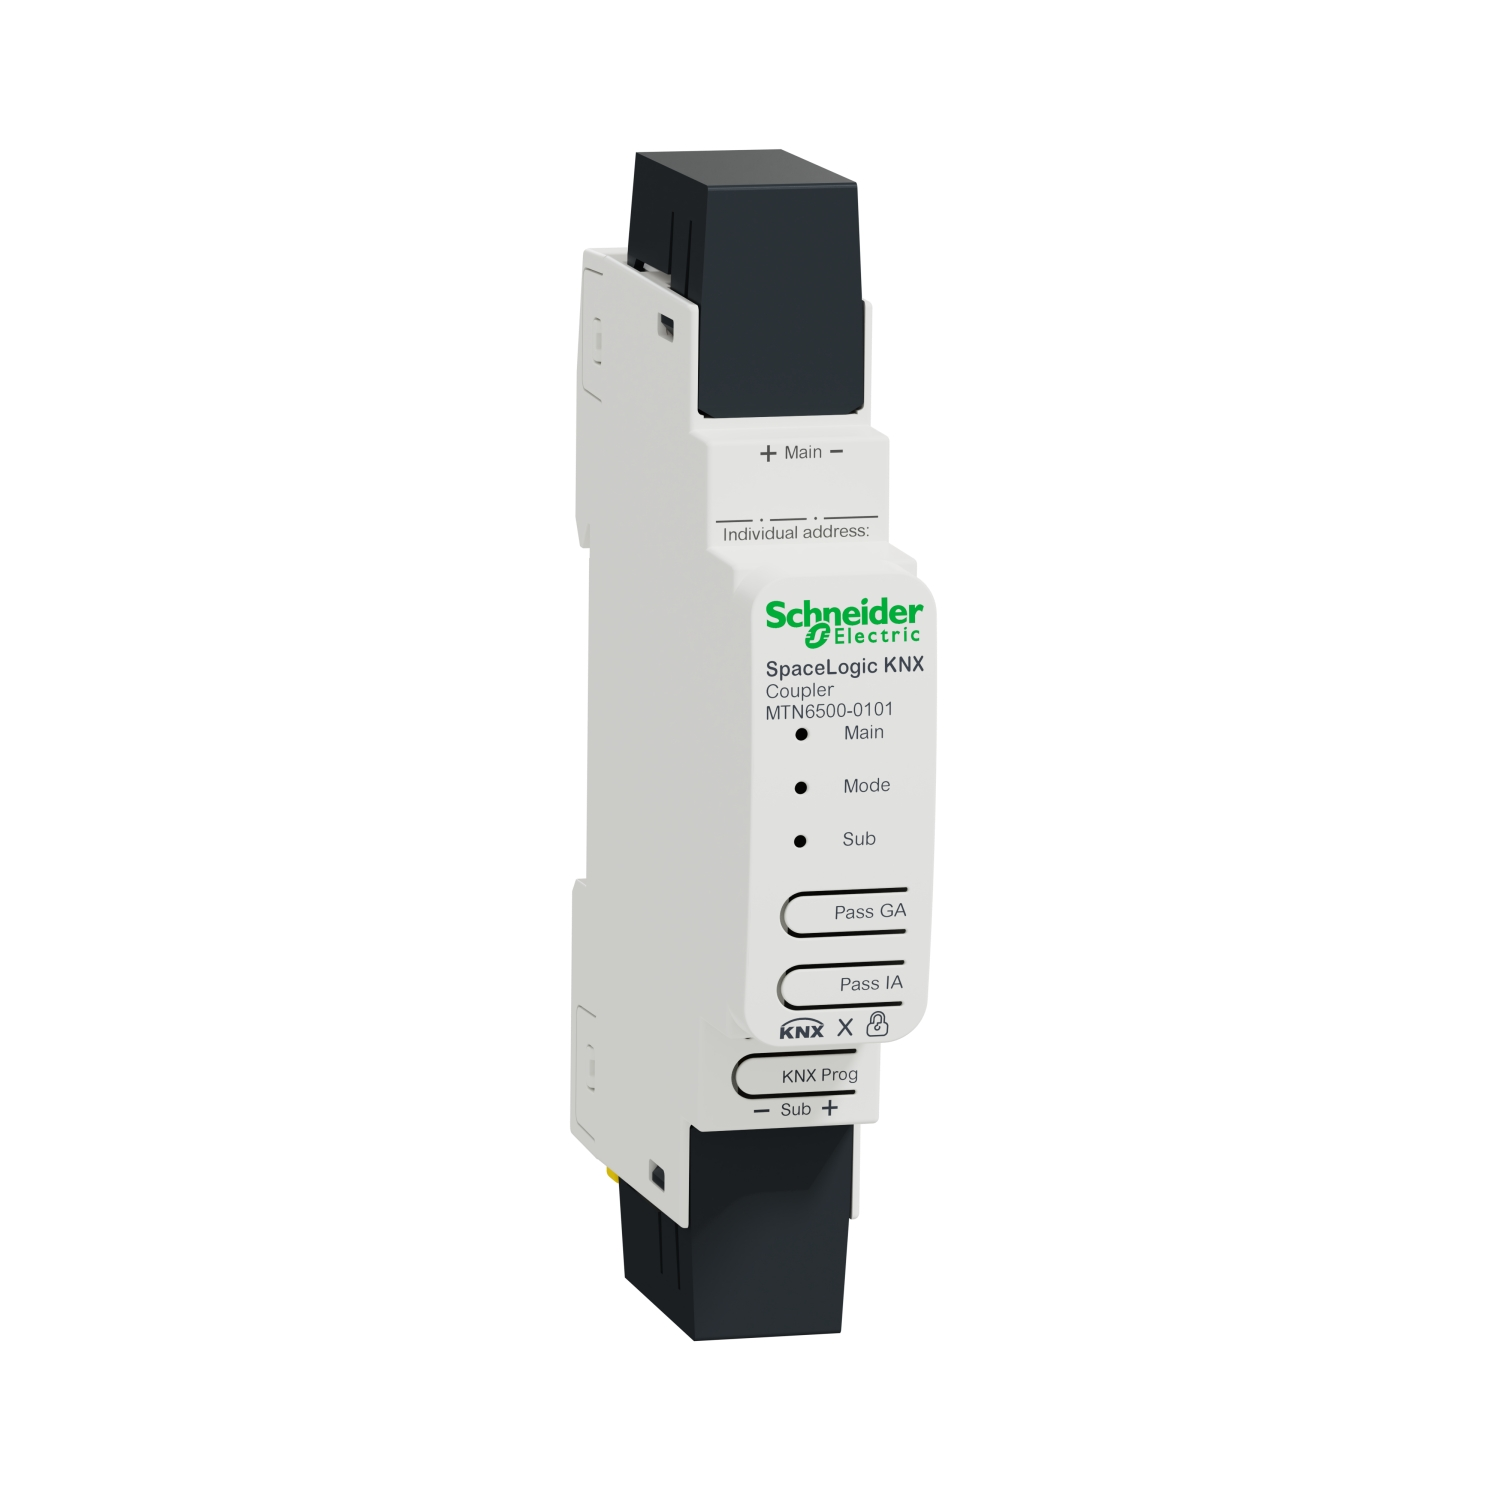
\includegraphics[scale=0.09]{image/MTN6500-0101.jpg}
		\caption{MTN6500-010 }
		\label{image:8}
\end{subfigure}

\begin{subfigure}{0.9\textwidth}
	\subsubsection{Termostat MTN6212-0325}
	Tento termostat slouží ke kontrole teploty pomocí ovladače v rámu okolo displaye s dalšími dvěmi volně nastavitelným dvojicemi tlačítek. Integrována je i sběrnicová spojka.  Display může zobrazovat aktuální i nastavenou teplotu, rychlost ventilátoru, zda probíhá ohřev či chlazení, čas apod.

	\noindent Tento projekt využívá jen ovladač v rámu a display, přičemž zařízení je napojeno na Fan coil akční člen. Display zobrazuje aktuální teplotu, nastavenou teplotu a jestli probíhá chlazení nebo ohřev.

			\centering
		\centering
		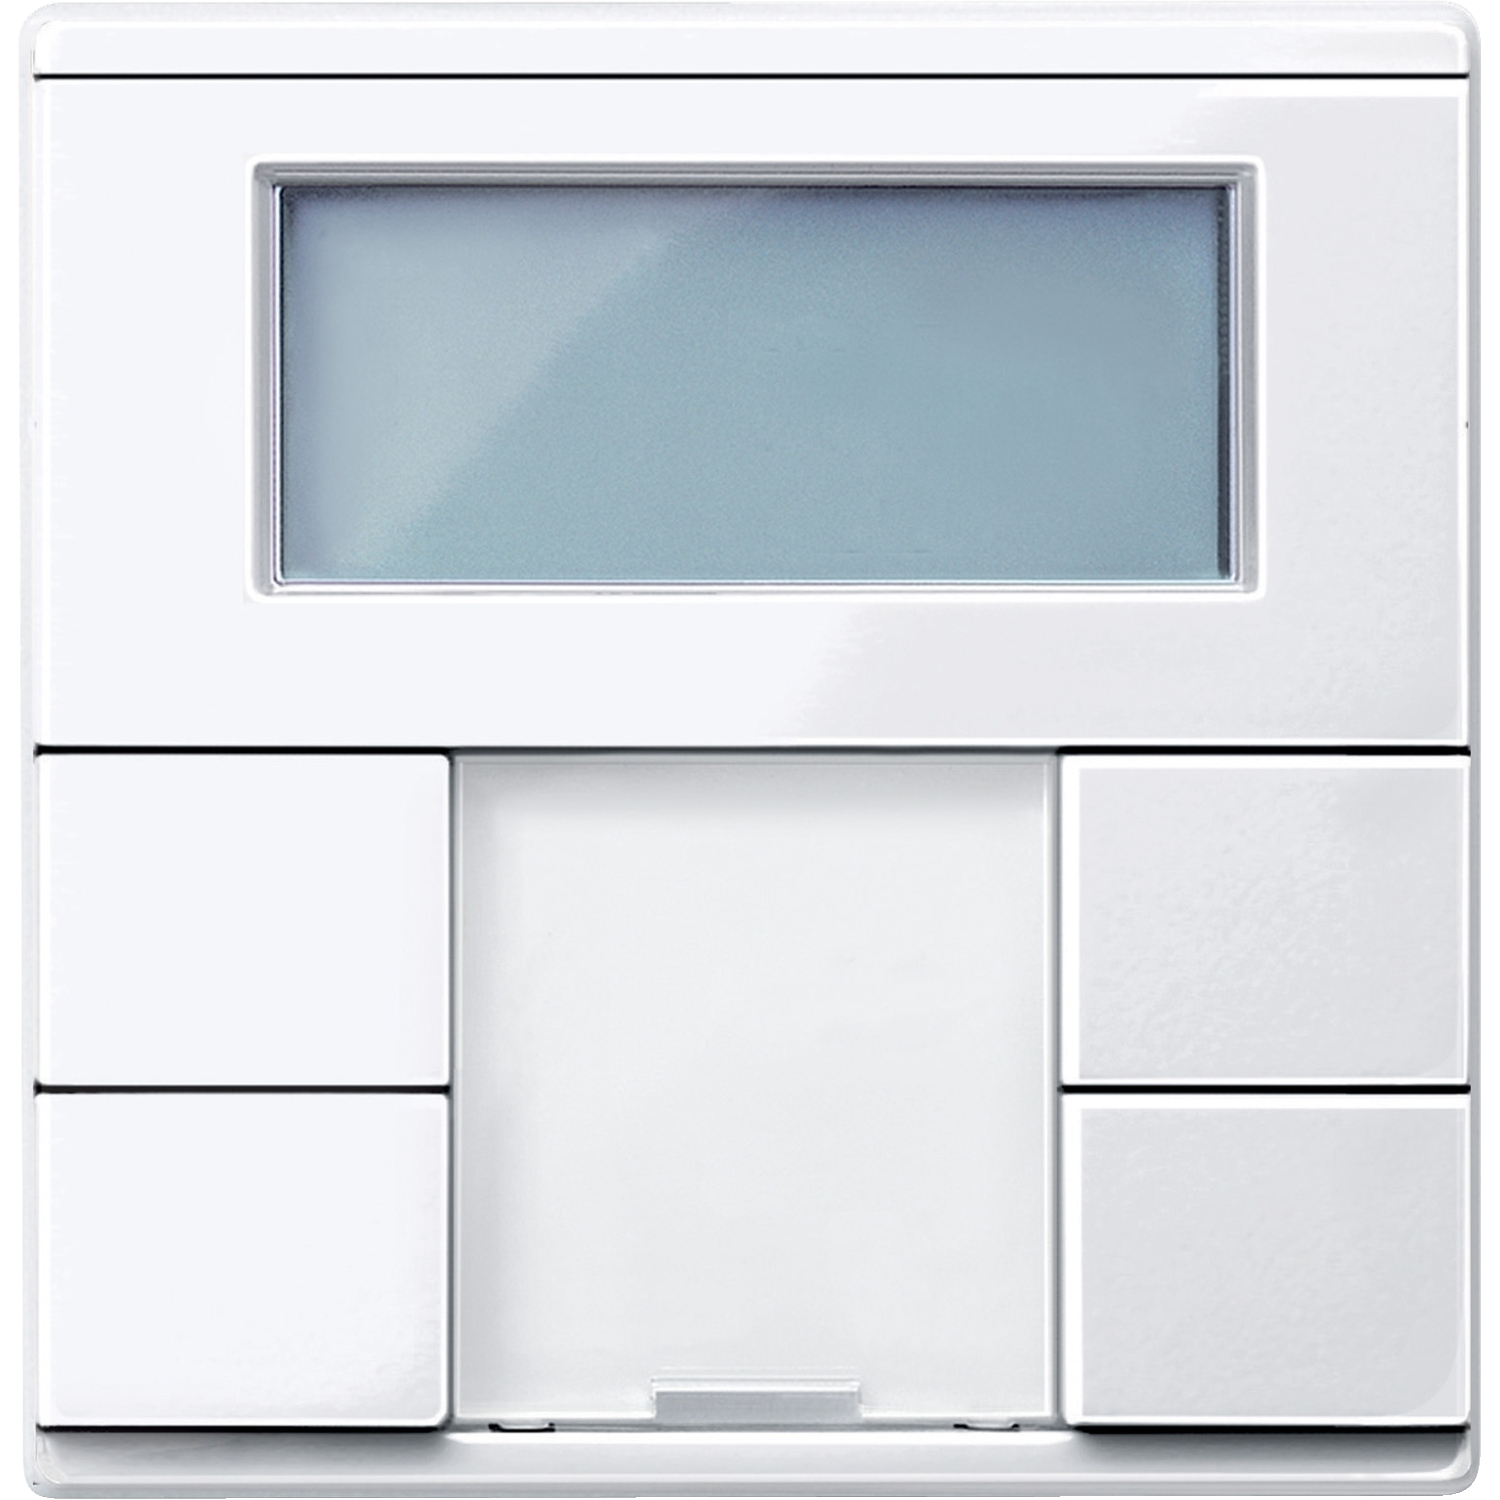
\includegraphics[scale=0.06]{image/MTN6212-0325.jpg}
		\caption{MTN6212-0325}
		\label{image:9}
\end{subfigure}
\end{figure}

\begin{figure}[h]
\centering
\begin{subfigure}{0.9\textwidth}
	\subsubsection{Čtyřpárový tlačítkový panel MTN617425}
	Jedná se o volně konfigurovatelný panel se čtyřmi páry tlačítek, která lze individuálně nastavit. Možné módy tlačítek jsou \textbf{toggle}, který po stisknutí změní hodnotu ze zapnuto na vypnuto a naopak, \textbf{switch}, kdy tlačítko pošle \textit{on} nebo \textit{off} signál podle toho který je nastaven, \textbf{dimming}, který slouží pro stmívání světel, \textbf{blind} sloužící pro ovládání pohybu a náklonu jednotlivých lamel žaluzií, \textbf{scene} pro aktivaci předem nastavených scén, neboli sekvence předem nastavených akcí, apod.

	\noindent Zde je panel 5.1.3 využit pro ovládání žaluzií pomocí akčního žaluziového členu 5.0.4, přičemž každé1. a 3. tlačítko v sloupci spouští pohyb nahoru a 2. a 4. pohyb dolů. U panelu 5.1.5 pak horní tři tlačítka v pravém sloupci přepínají stmívaná světla pod kontrolní jednotkou 5.0.5 a levý sloupec se stará o přepínání žárovek symbolizujících zásuvky pod akčním členem 5.0.3 módem toggle. Spodním tlačítkem v pravém sloupci lze nakonec zablokovat senzor pohybu 5.1.6.

		\centering
		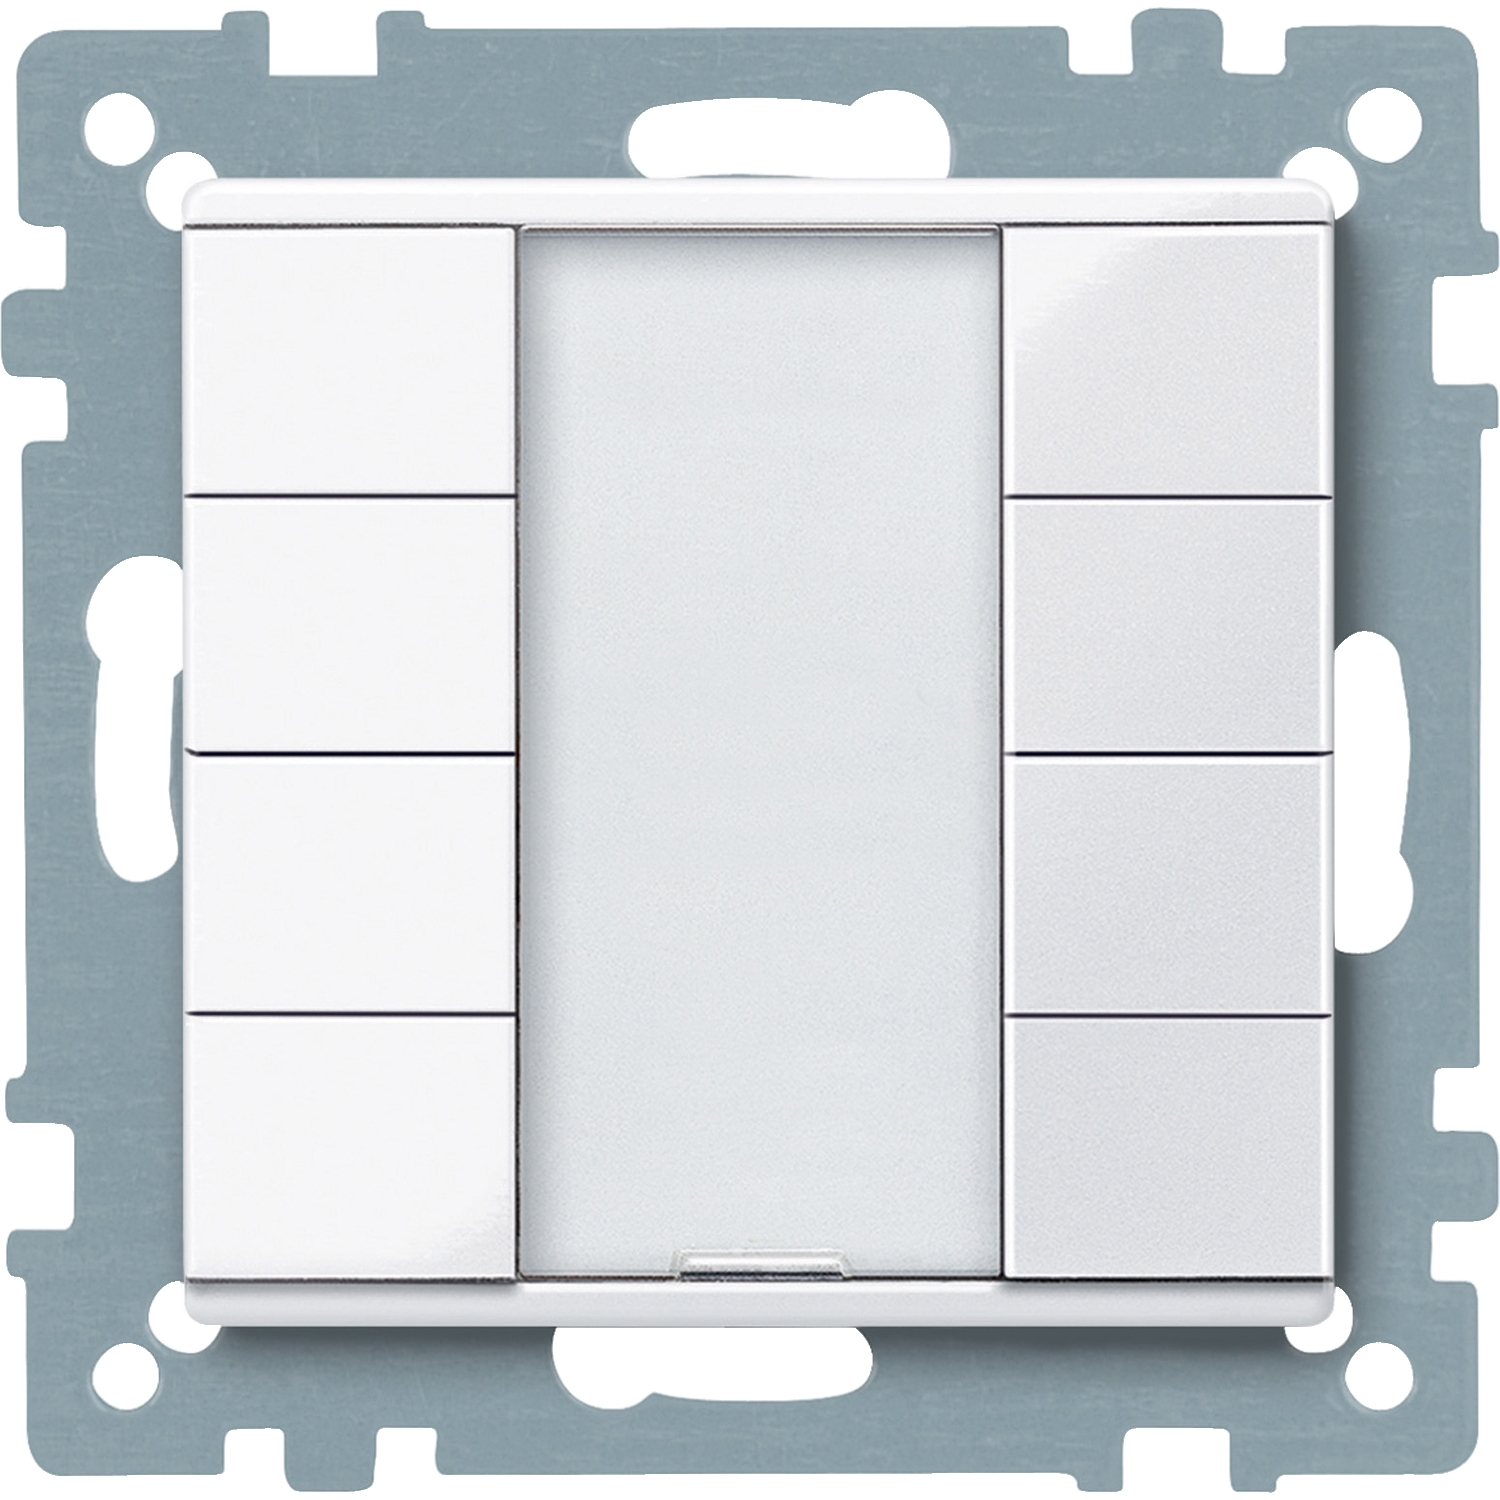
\includegraphics[scale=0.1]{image/MTN617425.jpg}
		\caption{MTN617425}
		\label{image:10}
\end{subfigure}

\begin{subfigure}{0.9\textwidth}
	\subsubsection{Jednopárový tlačítkový panel  MTN628019}
	Tento panel funguje na identickém principu jako panely 5.1.3 a 5.1.5. jediný rozdíl je v barvě LED diod, které svítí u tohoto panelu modře a u zbylých červeně, a počet tlačítek. Prodej byl ukončen 9.10. 2023

	\noindent Tento ovladač je užit k ovládání stmívaného světla v koupelně pomocí systému DALI přees DALI bránu 5.0.2.

		\centering
		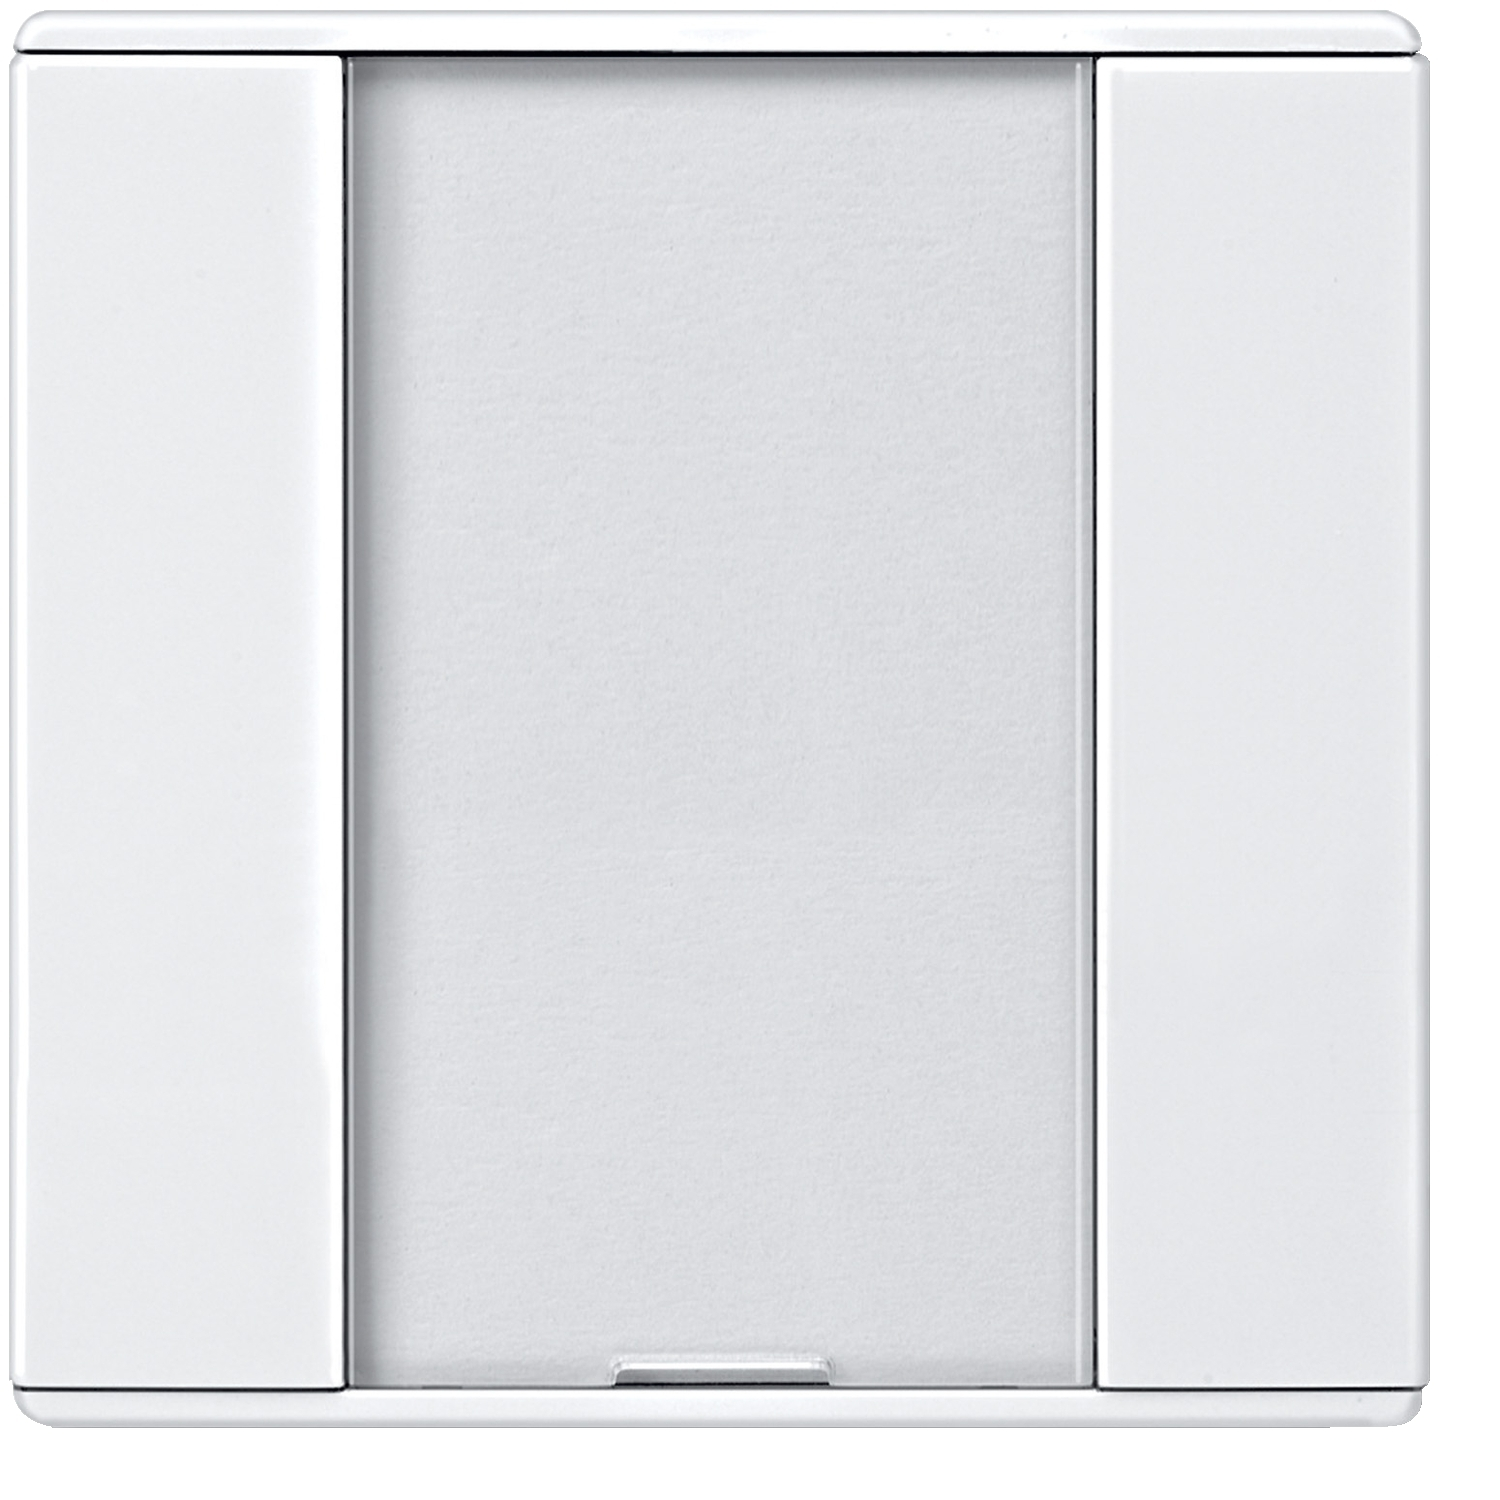
\includegraphics[scale=0.075]{image/MTN628019.jpg}
		\caption{MTN628019}
		\label{image:11}
\end{subfigure}

\begin{subfigure}{0.9\textwidth}
	\subsubsection{Detektor pohybu Argus 180 - MTN631625}
	Toto zařízení snímá pohyb pomocí infračerveného záření (PIR - passive infrared sensor). Tento senzor je určen pro použití uvnitř budov. Po detekci infračerveného záření, které je nejvylučovanější typ elektromagnetického záření při pokojové teplotě, pyroelektrickým filmem vyzařováno určité napětí, které aktivuje snímač. Jedná se o velmi úsporné řešení snímmání pohybu a je využíváno především v alarmech a spínání světla. Snímání probíhá v oblouku o úhlu 180° s dosahem 8 metrů pro výšku místění senzoru 1,1 metru. Citlivost snímání lze nastavit. Prodej byl ukončen 5.9. 2023.

	\noindent Tento senzor je v mém projektu využit k ovládání světla 2, které se ve vizualizaci nachází v předsíni.
		\centering
		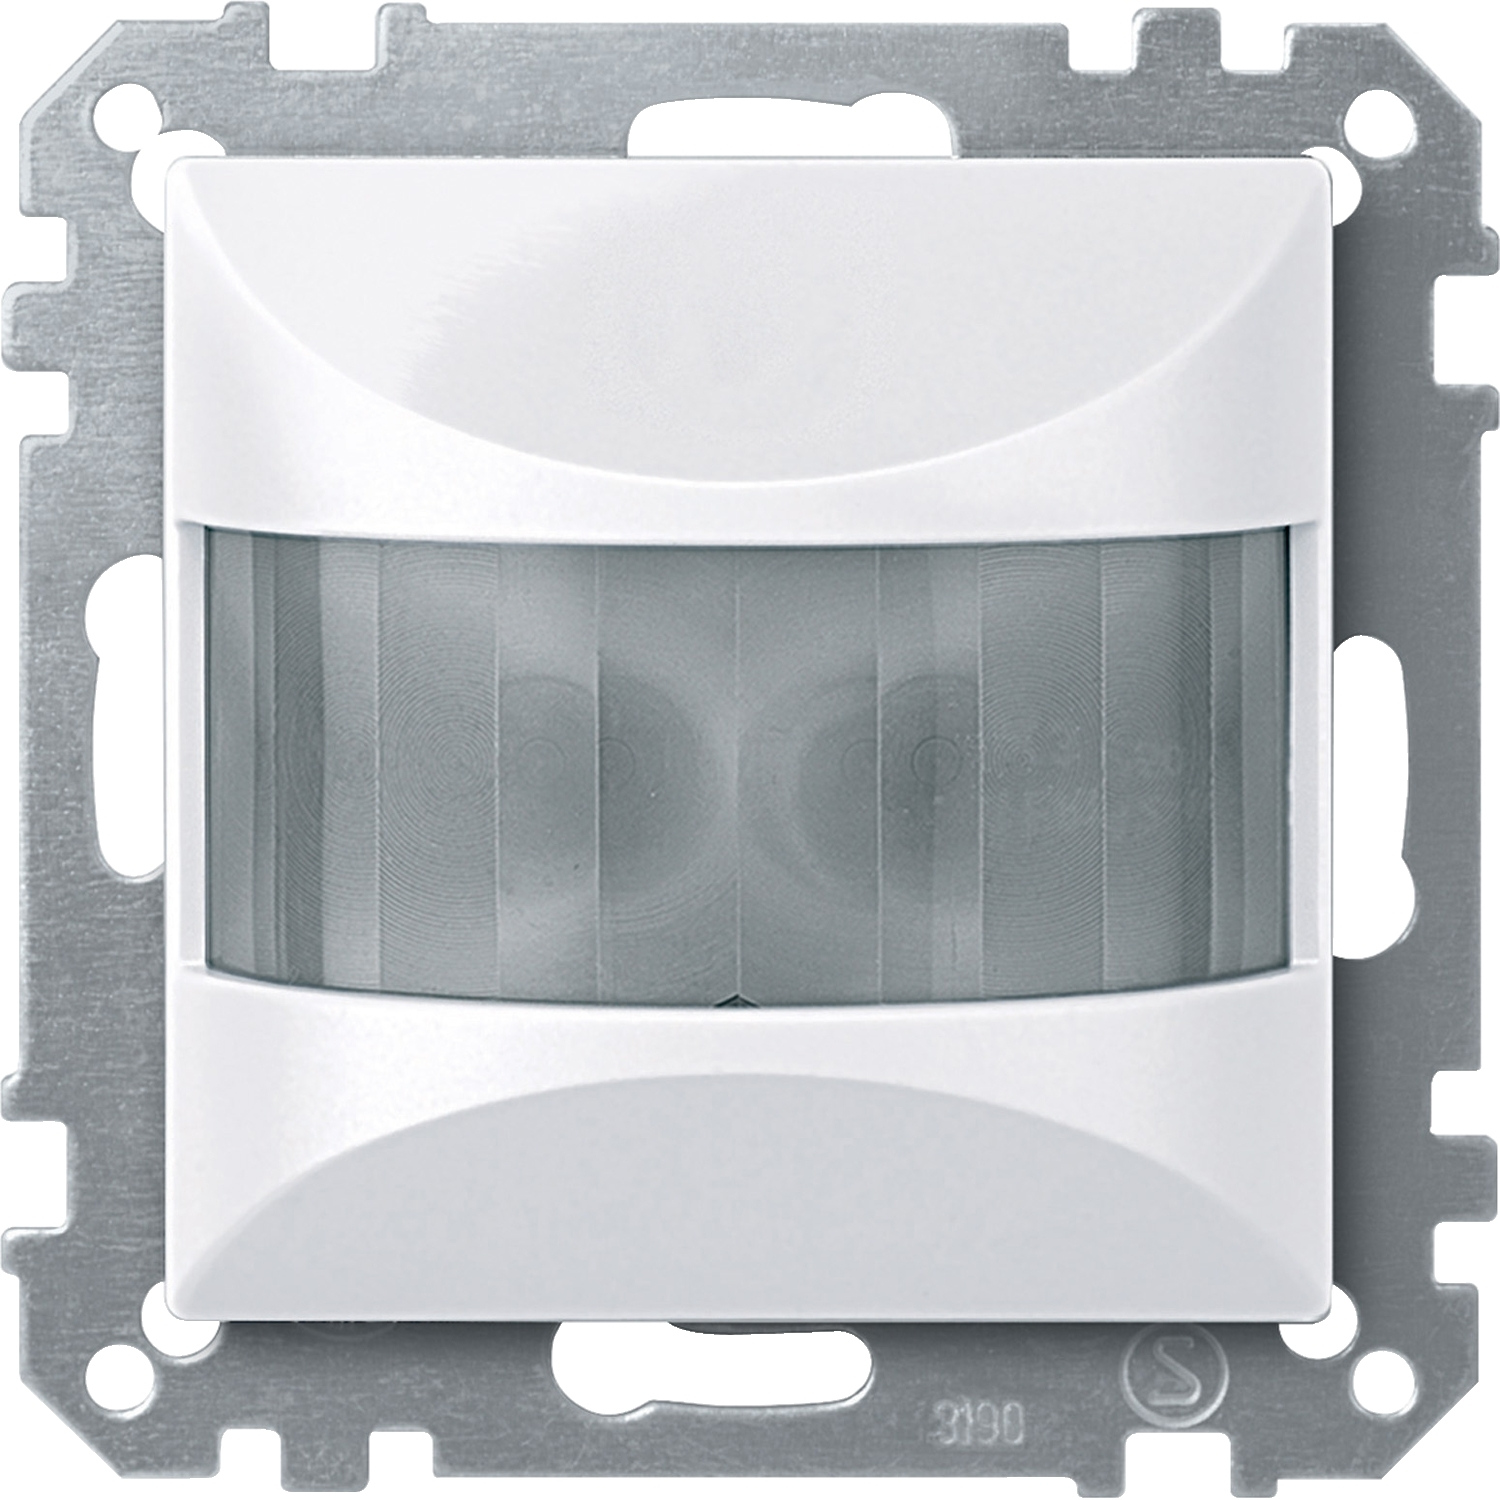
\includegraphics[scale=0.1]{image/MTN631625.jpg}
		\caption{MTN631625}
		\label{image:12}
\end{subfigure}

\begin{subfigure}{0.9\textwidth}
	\subsubsection{Detektor \texorpdfstring{CO\textsubscript{2}},, vlhkosti a teploty MTN6005-0001}
	Tímto zařízením lze měřit obsah \texorpdfstring{CO\textsubscript{2}},  pomocí vyhodnocení útlumu IR záření po průchodu vzduchem způsobeného obsahem oxidu uhličitého. Dále pak vlhkost, která se měří jako míra skutečného množství vzdušné vlhkosti v porovnání s maximální možnou vlhkostí při aktuální teplotě. Ta se pak měří pomocí termodiody, která propouští proud přímo úměrně k okolní teplotě.

	\noindent Všechny proměnné získané z tohoto přístroje zpracovávám a využívám je ve vizualizaci projektu.


		\centering
		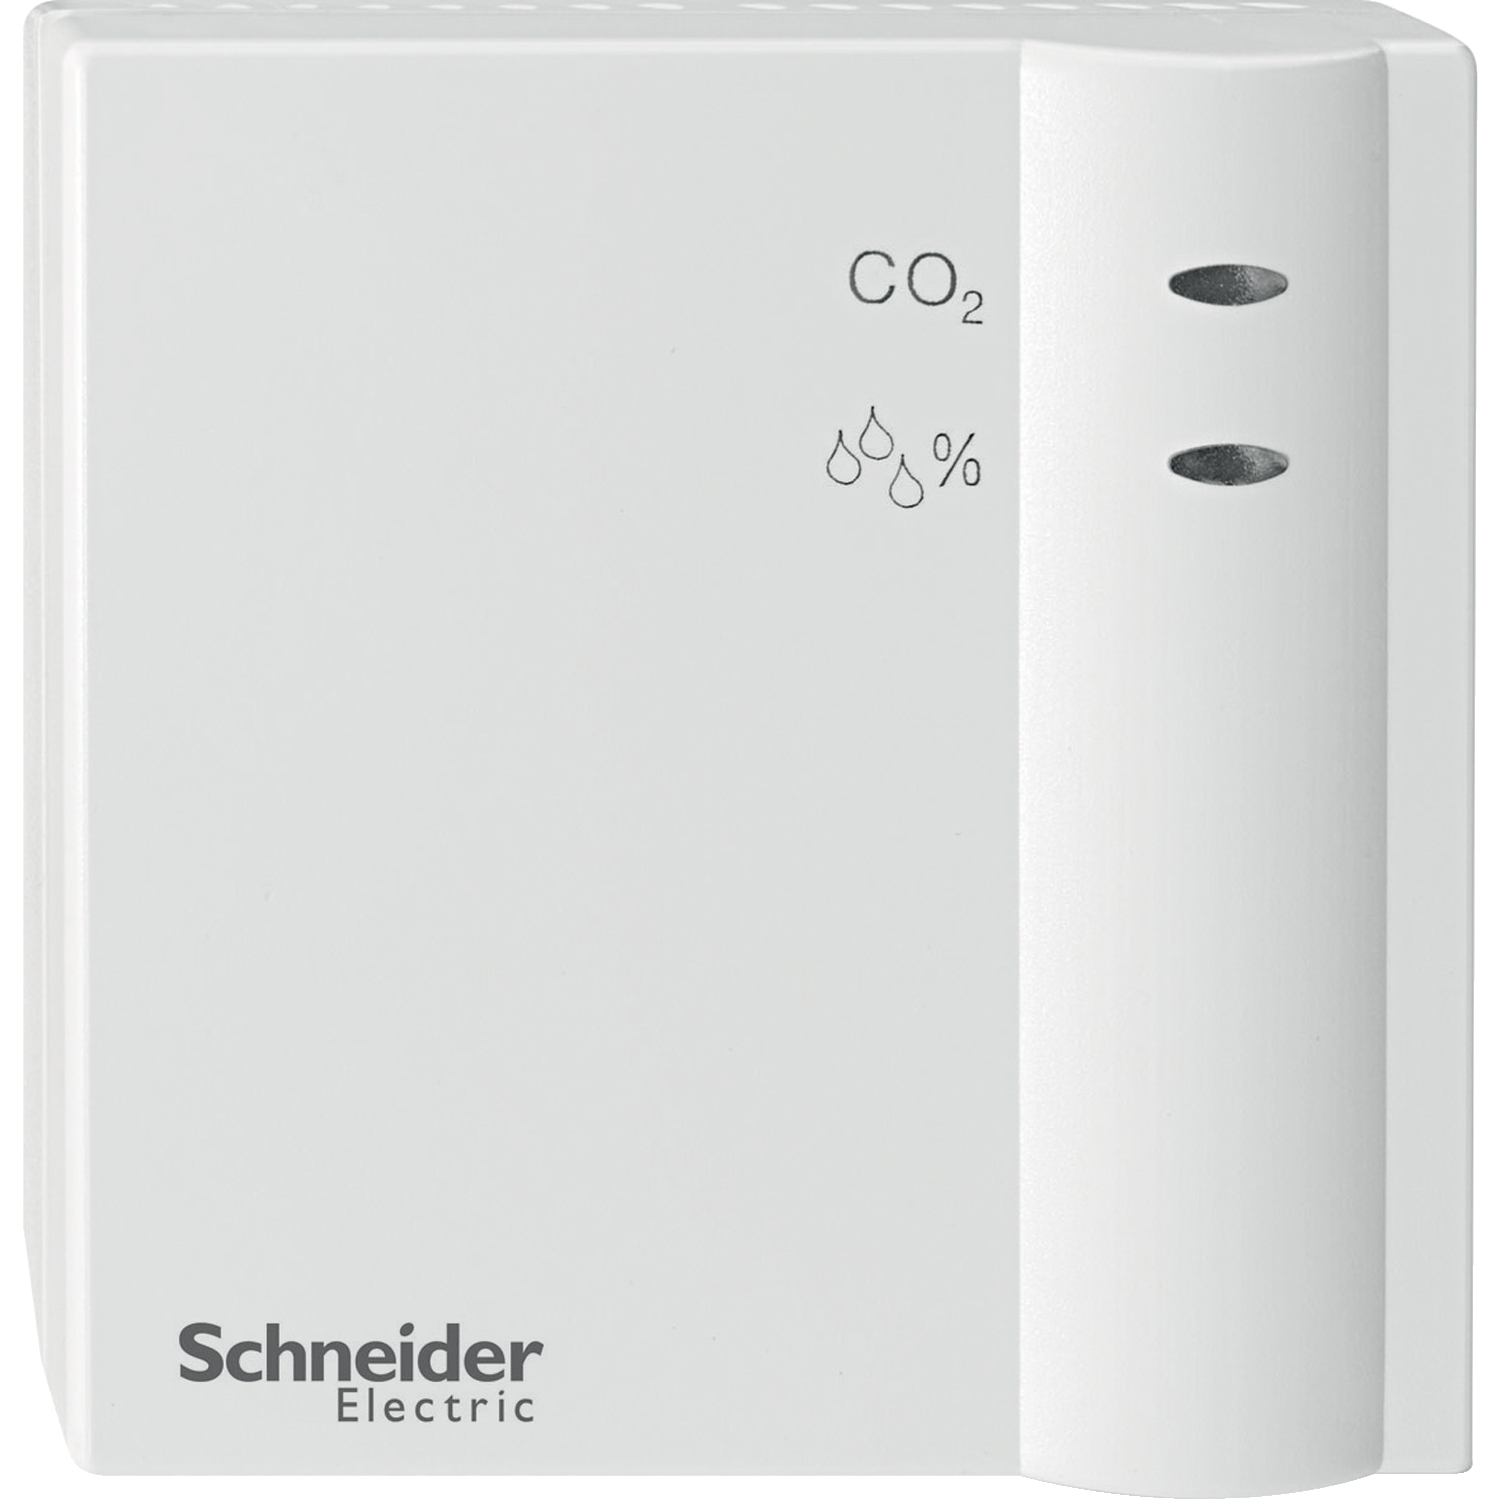
\includegraphics[scale=0.085]{image/MTN6005-0001.jpg}
		\caption{MTN6005-0001}
		\label{image:13}
\end{subfigure}
\end{figure}

\section{Konfigurace jednotlivých zařízení}
\label{sec:hw_conf}


\chapter{Vizualizace přes prohlížeč}	
	
	
\section[Tvorba prostředí]{Pokročilejší tipy}
	
\section{Nastavení komunikace s hardware}
	
	
	
	
\chapter{Umělá inteligence}

\section[Propojení]{Jak propojit Alexu od Amazonu}
\section{Vlastní konfigurace}
	
\chapter*{Závěr}

	%% literatura
	\begin{thebibliography}{99}
		\bibitem{KNX}KNX ASSOCIATION. \textit{KNX} [online]. [cit. 2023-12-26]. Dostupné z: \url{https://www.knx.org/knx-en/for-professionals/index.php}
		\bibitem{Loxone} LOXONE ELECTRONICS GMBH. \textit{Loxone} [online]. [cit. 2023-12-26]. Dostupné z: \url{https://www.loxone.com/cscz/}
		\bibitem{HA} \textit{Home Assistant} [online]. [cit. 2023-12-26]. Dostupné z: \url{https://www.home-assistant.io}
		\bibitem{BAC} BACNET COMMITTEE \textit{BACnet} [online]. [cit. 2023-12-26]. Dostupné z: \url{https://bacnetinternational.org}
		\bibitem{LW} ECHELONE CORPORATION \textit{LonWorks} [online]. [cit. 2023-12-26]. Dostupné z: \url{https://echelon.org}
		\bibitem{Teco} TECO A. S. \textit{Teco} [online]. [cit. 2023-12-26]. Dostupné z: \url{https://www.tecomat.cz}
		\bibitem{INELS} INELS S. R. O. \textit{iNELS} [online]. [cit. 2023-12-26]. Dostupné z: \url{https://www.inels.cz}
		\bibitem{sspuLogo} \textit{Střední škola průmyslová a umělecká Opava} [online]. [cit. 2023-11-11]. Dostupné z: \url{https://www.sspu-opava.cz}
		\bibitem{citacePRO}\textit{Citace PRO} [online]. Citace.com, 2020 [cit. 2020-08-31]. Dostupné z: \url{https://www.citacepro.com}
	\end{thebibliography}
	
	%% obrázky 
	\listoffigures
	
	%% tabulky
	\listoftables
	
	\appendix %% začínají přílohy
	
	\titleformat{\chapter}[block]{\scshape\bfseries\LARGE}{Příloha \thechapter}{10pt}{\vspace{0pt}}[\vspace{-22pt}] %% nastavení nadpisu u příloh
	
	
	\chapter{%Příloha A 
		Spot diagramy a další }
	
	
\end{document}